\chapter{ទ្រឹស្តីសុីនេទិចនៃឧស្ម័ន}
	\section{ទ្រឹស្តីសុីនេទិចនៃឧស្ម័ន}
	%
	\begin{definition}
		\emph{ទ្រឹស្តីសុីនេទិចនៃឧស្ម័នៈ} ជាការសិក្សាអំពីចលនារបស់ម៉ូលេគុលឧស្ម័ន ដែលស្ថិតក្នុងធុងដែលផ្ទុកវា។
	\end{definition}
	%
	\begin{figure}[H]
		\begin{subfigure}[t]{.5\textwidth}
			\centering
			\begin{tikzpicture}[scale=.8, magenta]
			\coordinate (O) at (0,0,0);
			\coordinate (A) at (0,\Width,0);
			\coordinate (B) at (0,\Width,\Height);
			\coordinate (C) at (0,0,\Height);
			\coordinate (D) at (\Depth,0,0);
			\coordinate (E) at (\Depth,\Width,0);
			\coordinate (F) at (\Depth,\Width,\Height);
			\coordinate (G) at (\Depth,0,\Height);
			\draw[->, -Stealth] (0,0,0) -- (4,0,0);
			\draw[->, -Stealth] (0,0,0) -- (0,4,0);
			\draw[->, -Stealth] (0,0,0) -- (0,0,4.5);
			\draw[gray,fill=orange!30] (O) -- (C) -- (G) -- (D) -- cycle;% Bottom Face
			\draw[fill=orange!20!white] (O) -- (A) -- (E) -- (D) -- cycle;% Back Face
			\draw[fill=red!10] (O) -- (A) -- (B) -- (C) -- cycle;% Left Face
			%\draw[fill=orange!40,opacity=1] (D) -- (E) -- (F) -- (G) -- cycle;% Right Face
			\fill [orange!50] (D) -- (E) -- (F) -- (G) -- cycle;% Right Face
			\pattern [pattern color=white, pattern=bricks,opacity=1] (D) -- (E) -- (F) -- (G) -- cycle;% Right Face
			\draw[fill=white!20,opacity=0.6] (C) -- (B) -- (F) -- (G) -- cycle;% Front Face
			\draw[fill=white!20,opacity=0.6] (A) -- (B) -- (F) -- (E) -- cycle;% Top Face
			\shade [ball color = green, opacity = 1] (-.5,1) circle (.2cm);
			\draw [->, -Latex, line width=1.5pt] (-.3,1) --(1,1.5);
			\draw [dashed, gray] (-.3,1) -- (2.5,1);
			\coordinate[label = right:$\overrightarrow{v}$] ($v$) at (.8,1.5);
			\coordinate[label = above:$m_{0}$] ($m_{0}$) at (-.5,1); 
			\draw (5,2) node {\text{\koc ផ្ទៃខាងនៃធុង}}; 
			\coordinate[label = right:$y$] ($y$) at (.1,0,4.5); 
			\coordinate[label = below:$x$] ($x$) at (3.8,0,0);
			\coordinate[label = right:$z$] ($z$) at (0,3.8,0); 
			\draw [->, -Latex, line width=1.0pt] (4,1.8) --(2.5,1);
			\end{tikzpicture}
			\subcaption{\koc ធុងផ្ទុកឧស្ម័ន}
		\end{subfigure}
		\begin{subfigure}[t]{.5\textwidth}
			\centering
			\begin{tikzpicture}[scale=0.8]
			\begin{scope}[every node/.append style={
				yslant=0,xslant=0},yslant=0,xslant=2.5
			]
			\shade[bottom color = orange!30, top color = white] (-12.54, 5)
			rectangle +(0.1, 1.1);
			\shade[bottom color = orange!30, top color = white] (-12.48,5)
			rectangle +(0.5,1.1);
			\shade[bottom color = orange!30, top color = white] (-12, 4.98)
			rectangle +(0.1, 1.1);
			\end{scope}
			
			\begin{scope}[every node/.append style={
				yslant=0,xslant=0},yslant=0.4,xslant=0
			]
			\fill[orange!50, left color = orange!50, right color = orange!10!white]
			(0.54,-0.26) rectangle +(2.8,5.03);
			\pattern [pattern color=white, pattern=bricks] (0.54,-0.26) rectangle +(2.8,5.03);
			
			\end{scope}
			
			\pgfmathsetseed{10}
			
			\foreach \i in {1,2,...,10}{
				\pgfmathsetmacro{\x}{(rand*0.5 + 1)*3 - 0.5}
				\pgfmathsetmacro{\y}{(rand*0.5 + 1)*4.7-1.2}
				\pgfmathsetmacro{\opacVal}{0.95*(\x-2.5)/4 + rand*0.05}
				\pgfmathsetmacro{\opacVal}{rand*0.5+1}
				\shade [ball color = green, opacity = \opacVal] (\x,\y) circle (0.1);
			}
			
			\fill [fill = magenta!60,rounded corners= 0.6] (-0.05,-0.05)
			rectangle +(0.6,5.05);
			\fill [fill = orange!60] (0,0) rectangle +(0.5,4.95);
			\end{tikzpicture}
			\subcaption{\koc ផ្ទៃខាងនៃធុង}
		\end{subfigure}
	\end{figure}
	\begin{itemize}
		\item ម៉ូលេគុលឧស្ម័នទាំងអស់ធ្វើចលនាឥតឈប់ឈរ និងគ្មានសណ្តាប់ធ្នាប់។
		\item គ្រប់ការទង្គិចរបស់ម៉ូលេគុលជាទង្គិចខ្ទាត។
		\item គេសន្មតថាម៉ូលេគុលនីមួយៗមានល្បឿនថេរជានិច្ច និងអាចអនុវត្តច្បាប់ញ៉ូតុនបានគ្រប់ពេល។
		\item គេចាត់ទុកម៉ូលេគុលឧស្ម័នជាចំណុចរូបធាតុ ព្រោះវិមាត្ររបស់ម៉ូលេគុលនីមួយៗតូចធៀបនឹងលំហអន្តរម៉ូលេគុល។
		\item ថាមពលសុីនេទិចមធ្យមនៃម៉ូលេគុលសមាមាត្រនឹងសីតុណ្ហភាព។
	\end{itemize}
	\section{សម្ពាធក្នុងទ្រឹស្តីសុីនេទិចនៃឧស្ម័ន}
	\quad យើងសិក្សាចលនាម៉ូលេគុលក្នុងធុងមួយ។ យើងបានសម្ពាធដែលសង្តត់លើផ្ទៃធុងគឺជាកម្លាំងទង្គិចរបស់ចលនាម៉ូលេគុល
	\begin{align*}
	\text{យើងបាន}\quad :&\quad P=\frac{F}{A}\quad \text{ដោយ}: \quad F=m\frac{\Delta \upsilon_{x}}{\Delta t}=\frac{m\times2\upsilon_{x}}{\dfrac{2L}{\upsilon_{x}}}=\frac{m\upsilon^{2}_{x}}{L}\\
	\text{យើងបាន}\quad :&\quad P=\frac{m\upsilon^{2}_{x}}{AL}=\frac{m\upsilon^{2}_{x}}{V}\\
	\text{តែ}\quad :&\quad \left(\upsilon^{2}\right)_{av}=\left(\upsilon^{2}_{x}\right)_{av}+\left(\upsilon^{2}_{y}\right)_{av}+\left(\upsilon^{2}_{z}\right)_{av}=3\left(\upsilon^{2}_{x}\right)_{av}\\\text{ដែល}\quad :&\quad \left(\upsilon=\upsilon_{x}=\upsilon_{y}=\upsilon_{z}=\text{ថេរ}\right)\\
	\text{នាំឲ្យ}\quad :&\quad \left(\upsilon^2_{x}\right)_{av}=\frac{1}{3}\left(\upsilon^2\right)_{av}\\
	\text{យើងបានសម្ពាធលើផ្ទៃខាងនីមួយៗ កំណត់ដោយៈ}\quad :&\quad P=\frac{1}{3}\times\frac{m}{V}\left(\upsilon^{2}\right)_{av}\quad \text{ឬ}\quad P=\frac{1}{3}\rho\left(\upsilon^{2}\right)_{av}\\
	\text{ដែល}\quad :&\quad \rho =\frac{m}{V}\left(\text{ម៉ាសមាឌ}\right)\\
	\text{ម្យ៉ាងទៀត}\quad :&\quad m=m_{0}N\\
	\text{យើងបាន}\quad :&\quad P=\frac{1}{3}\times\frac{Nm_{0}}{V}\left(\upsilon^{2}\right)_{av}=\frac{2N}{3V}\times\frac{1}{2}m_{0}\left(\upsilon^2\right)_{av}\\
	\text{ដូចនេះ}\quad :&\quad P=\frac{2}{3}\times\frac{N}{V}K_{av}
	\end{align*}
	\section{ថាមពលសុីនេទិច និងសីតុណ្ហភាព}
	 \subsection{សមីការភាពនៃឧស្ម័នបរិសុទ្ធៈ} 
	 	\begin{multicols}{2}
	 	តាមពិសោធន៍បង្ហាញថាៈ
			\begin{itemize}
				\item សម្ពាធសមាមាត្រនឹងសីតុណ្ហភាព: \quad $P\sim T$
				\item សម្ពាធសមាមាត្រនឹងចំនួនម៉ូលេគុល: \quad $P\sim N$
				\item សម្ពាធច្រាសសមាមាត្រនឹងមាឌ: \quad $P\sim\frac{1}{V}$
			\end{itemize}
			\begin{figure}[H]
				\centering
				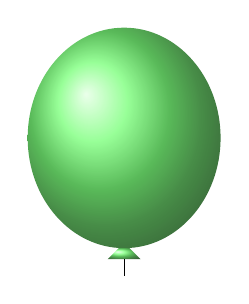
\begin{tikzpicture}[scale=.7]
					\begin{scope}
						\tikzstyle{balloon}=[ball color=green!60];    
						\shade[balloon, opacity=0.90] ellipse (1.75 and 2);
						\shade[balloon, opacity=0.90] (-.1,-2) -- (-.3,-2.2) -- (.3,-2.2) -- (.1,-2) -- cycle;
						\draw (0,-2.2) -- (0,-2.5);
					\end{scope}
				\end{tikzpicture}
				\caption{បាឡុងរាងស៊្វែផ្ទុកឧស្ម័ន}
			\end{figure}
		\end{multicols}
		\begin{align*}
			\text{យើងបាន}\quad :& \quad P\sim \frac{NT}{V}\quad \text{ឬ}\quad P=k_{B}\frac{NT}{V}\quad \text{នោះ}\quad PV=Nk_{B}T\\\text{ដែល}\quad :&\quad k_{B}=1.38\times10^{-23}J/K\left(\text{ថេរបុលស្មាន់}\right)\\
			\text{តែ}\quad :&\quad N=nN_{A}\quad \text{នោះ}\quad PV=nk_{B}N_{A}T\\
			\text{តាង}\quad :&\quad R=k_{B}N_{A}\quad\text{ដែល}\quad N_{A}=6.02\times10^{23}\text{ម៉ូលេគុល}/mol\left(\text{ចំនួនអាវ៉ូកាដ្រូ}\right)\\
			\text{ដូចនេះ}\quad :&\quad PV=k_{B}NT=nRT
		\end{align*}
		\subsection{សមីការបម្រែបម្រួលភាពនៃឧស្ម័នបរិសុទ្ធៈ} បើឧស្ម័នប្រែប្រួលភាព ពីភាពដើម $1$ ទៅភាពស្រេច $2$ យើងបានៈ
		\begin{itemize}
			\begin{multicols}{2}
				\item នៅភាពដើម $1$: $P_{1}V_{1}=nRT_{1}$ ឬ $\frac{P_{1}V_{1}}{T_{1}}=nR$
				\item នៅភាពស្រេច $2$: $P_{2}V_{2}=nRT_{2}$ ឬ $\frac{P_{2}V_{2}}{T_{2}}=nR$
			\end{multicols}
		\end{itemize}
		\begin{align*}
		\text{យើងបាន}\quad :&\quad \frac{P_1V_1}{T_1}=\frac{P_2V_2}{T_2}=nR=\text{ថេរ}\\
		\text{ច្បាប់ប៊យ-ម៉ារ្យ៉ូត}\quad :&\quad P_{1}V_{1}=P_{2}V_{2}\quad \left(\text{សីតុណ្ហភាពថេរ} T_{1}=T_{2}\right)\\
		\text{ច្បាប់សាល}\quad :&\quad \frac{P_1}{T_1}=\frac{P_2}{T_2}\quad \left(\text{មាឌថេរ} V_{1}=V_{2}\right)\\
		\text{ច្បាប់កេលុយសាក់}\quad :&\quad \frac{P_1V_1}{T_1}=\frac{P_2V_2}{T_2}\\
		\end{align*}
		\subsection{ថាមពលសុីនេទិច និងសីតុណ្ហភាពៈ}
		\begin{enumerate}[m]
			\item {\kml \color{magenta} តម្លៃថាមពលសុីនេទិចមធ្យមនៃម៉ូលេគុលឧស្ម័នៈ}
			\begin{align*}
			\text{តាមសម្រាយបញ្ជាក់ខាងលើ}\quad :&\quad P=\frac{2}{3}\times\frac{N}{V}K_{av}\quad\\ \text{យើងបានៈ}\quad :&\quad PV=\frac{2}{3}NK_{av}\\
			\text{នាំឲ្យ}\quad :&\quad K_{av}=\frac{3}{2}\times\frac{PV}{N}=\frac{3}{2}k_{B}T\\\quad\text{ព្រោះ}\quad :& \quad \frac{PV}{N}=k_{B}T\\
			\text{ដូចនេះ តម្លៃថាមពលសុីនេទិចមធ្យមនៃម៉ូលេគុលឧស្ម័នគឺៈ}\quad :& \quad K_{av}=\frac{3}{2}k_{B}T=\frac{3}{2}\left(\frac{PV}{N}\right)
			\end{align*}
			\item {\kml \color{magenta} តម្លៃថាមពលសុីនេទិចសរុបនៃម៉ូលេគុលឧស្ម័នៈ}
			\begin{align*}
			\text{យើងមាន}\quad :&\quad K_{av}=\frac{3}{2}k_{B}T\\
			\text{នាំឲ្យ}\quad :&\quad K=N\times K_{av}=\frac{3}{2}Nk_{B}T=\frac{3}{2}nRT\\
			\text{ដូចនេះ តម្លៃថាមពលសុីនេទិចសរុបនៃម៉ូលេគុលឧស្ម័នគឺៈ}\quad :& \quad K=\frac{3}{2}Nk_{B}T=\frac{3}{2}nRT=\frac{3}{2}PV
			\end{align*}
		\end{enumerate}
		\subsection{ល្បឿនប្ញសការេនៃការេល្បឿនមធ្យមៈ}
		\begin{align*}
		\text{យើងមាន}\quad :& \quad K_{av}=\frac{3}{2}k_{B}T=\frac{1}{2}m_{0}\left(\upsilon^{2}\right)_{av}\\
		\text{នាំឲ្យ}\quad :&\quad \sqrt{\left(\upsilon^{2}\right)_{av}}=\sqrt{\frac{3k_{B}T}{m_{0}}}\\
		\text{តាង}\quad :& \quad \upsilon_{rms}=\sqrt{\left(\upsilon^{2}\right)_{av}}=\sqrt{\frac{3k_{B}T}{m_{0}}}=\sqrt{\frac{3RT}{M}}\\
		\text{ដូចនេះ ល្បឿនប្ញសការេនៃការេល្បឿនមធ្យមគឺៈ}\quad :& \quad \upsilon_{rms}=\sqrt{\frac{3k_{B}T}{m_{0}}}=\sqrt{\frac{3RT}{M}}
		\end{align*}
		\begin{remark}
			\begin{enumerate}[m]
				\item ល្បឿនមធ្យមៈ $\upsilon_{av}=\frac{\upsilon_{1}+\upsilon_{2}+\upsilon_{3}+\cdots+\upsilon_{N}}{N}$\quad ដែល\quad $\upsilon_{av}$ គិតជា $m/s$\\
				$\left(\upsilon_{av}\right)^2=\left(\overline{\upsilon}\right)^2=\left(\frac{\upsilon_1+\upsilon_2+\upsilon_3+\cdots+\upsilon_{N}}{N}\right)^2$ ល្បឿនមធ្យមលើកជាការេ\\
				$\left(\upsilon^2\right)_{av}=\upsilon^2_{rms}=\frac{\upsilon^2_1+\upsilon^2_2+\upsilon^2_3+\cdots+\upsilon^2_{N}}{N}$ តម្លៃមធ្យមនៃការេល្បឿន​\\
				\item ល្បឿនប្ញសការេនៃការេល្បឿនមធ្យមៈ $\upsilon_{rms}=\sqrt{\left(\upsilon^2\right)_{av}}=\sqrt{\frac{\upsilon^2_{1}+\upsilon^2_{2}+\upsilon^2_{3}+ \cdots+\upsilon^2_{N}}{N}}$\quad \\ដែល\quad $\upsilon_{rms}$ គិតជា $m/s$ \quad ​និង
				$\upsilon^2_{rms}=\left(\upsilon^2\right)_{av}$
				\item ម៉ាសមាឌ ឬដង់សុីតេមាឌនៃឧស្ម័នៈ $\rho=\frac{m}{V}=\frac{m_{0}N}{V}$\quad ដែល\quad $\rho$ គិតជា $\left(kg/m^3\right)$\\ $m$ ជាម៉ាសឧស្ម័ន គិតជា $\left(kg\right)$\\ $m_{0}$ ម៉ាសមូលេគុល គិតជា $\left(kg\right)$ 
				\\ $V$ មាឌឧស្ម័ន គិតជា $\left(m^3\right)$
				\item ចំនួនម៉ូលៈ $n=\frac{m}{M}=\frac{N}{N_{A}}=\frac{V}{V_{mol}}$\quad ដែល\quad $M$ ម៉ាសម៉ូលគិតជា $\left(kg/mol\right)$\\
				$N$ ចំនួនម៉ូលេគុលសរុប\\
				$V_{mol}$ ជាមាឌឧស្ម័នក្នុងមួយម៉ូល $\left(m^3/mol\right)$\\
				$V$ មាឌឧស្ម័ន $\left(m^3\right)$
				\item ចំនូនម៉ូលេគុលសរុបនៃឧស្ម័នៈ $N=\frac{m}{m_{0}}=nN_{A}=\frac{m}{M}\times N_{A}$ ដែល $n$ ចំនួនម៉ូល​ គិតជា $\left(mol\right)$
				\item មាឌម៉ូលនៃឧស្ម័នក្នុងលក្ខខ័ណ្ឌគំរូដែលមានសម្ពាធ $P_{0}=1atm$ និងសីតុណ្ហភាព $T=273K$ \\គឺៈ $V_{mol}=22.4\times10^{-3}m^3/mol$
				\item ល្បឿននៃចលនាត្រង់ស្មើៈ(បម្លាស់ទី=ល្បឿន$\times$ រយៈពេល) $x=\upsilon\times\Delta t$
			\end{enumerate}
		\end{remark}